\section{Anhang}\label{sec:anhang}
\subsubsection*{Darstellung der vom Assistenten bereitgestellten Rohdaten zum ersten Versuchsteil}
\begin{figure}[H]
	\centering
	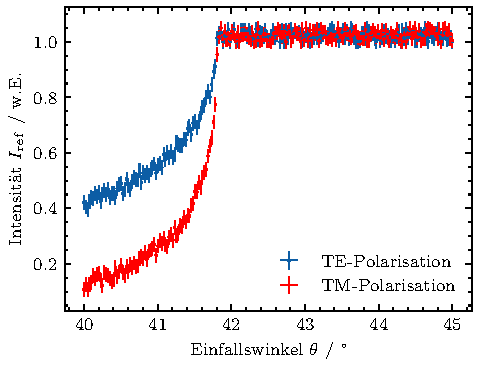
\includegraphics[width=0.4\linewidth]{../figs/referenz.pdf}
	\caption{Vom Assistenten bereitgestellte Rohdaten der Referenzmessung für ein unbeschichtetes Deckglas für TM- und TE-Polarisation (die Winkelunsicherheiten sind für diesen Winkelbereich zu klein, um erkennbar zu sein).}
	\label{fig:referenz}
\end{figure}
\begin{figure}[H]
    \centering
    \begin{subfigure}{0.4\textwidth}
        \centering
        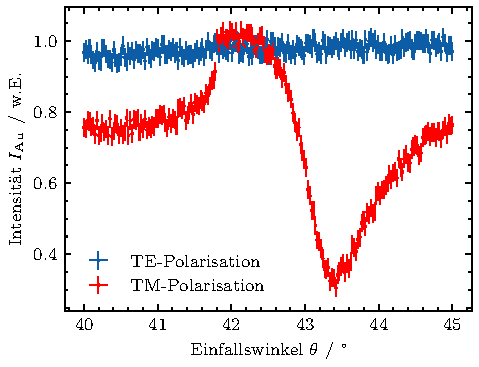
\includegraphics[width=\linewidth]{../figs/au1}
        \caption{Goldfilm 1}
    \end{subfigure}
    \begin{subfigure}{0.4\textwidth}
        \centering
        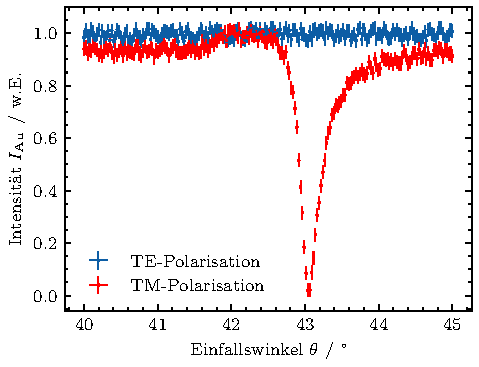
\includegraphics[width=\linewidth]{../figs/au2}
        \caption{Goldfilm 2}
    \end{subfigure}
    \begin{subfigure}{0.4\textwidth}
        \centering
        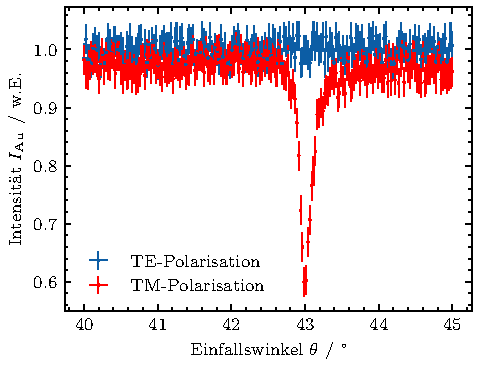
\includegraphics[width=\linewidth]{../figs/au3}
        \caption{Goldfilm 3}
    \end{subfigure}
    \begin{subfigure}{0.4\textwidth}
        \centering
        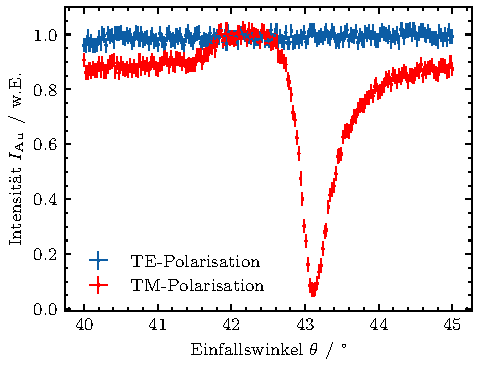
\includegraphics[width=\linewidth]{../figs/au4}
        \caption{Goldfilm 4}
    \end{subfigure}
    \caption{Vom Assistent bereitgestellte Rohdaten der Reflexionsmessungen an vier Goldfilmen für TM- und TE-Polarisation (die Winkelunsicherheiten sind für diesen Winkelbereich zu klein, um erkennbar zu sein).}\label{fig:gold}
\end{figure}